\documentclass{article}[12pt]

% useful packages
\usepackage{titlesec}
\usepackage{fullpage}
\usepackage{amsmath,amssymb,amsthm,amsfonts}
\usepackage{graphicx}
\usepackage{enumerate}
\usepackage{algorithm,algorithmic}
\usepackage{xcolor}
\usepackage{bbm}
\usepackage{url,hyperref}
\usepackage{dirtree}

% theorem type environments
\newtheorem{thm}{Theorem}
\newtheorem{prop}{Proposition}
\newtheorem{lemma}{Lemma}
\newtheorem{cor}{Corollary}
\newtheorem{defn}{Definition}
\newtheorem{assump}{Assumption}
\newtheorem{example}{Example}
\newtheorem{conjecture}{Conjecture}

% frequently used symbols
\newcommand{\bE}{\mathbb{E}}
\newcommand{\bP}{\mathbb{P}}
\newcommand{\bQ}{\mathbb{Q}}
\newcommand{\bR}{\mathbb{R}}
\newcommand{\bS}{\mathbb{S}}
\newcommand{\bN}{\mathbb{N}}
\newcommand{\bZ}{\mathbb{Z}}
\newcommand{\sC}{{\mathcal C}} 
\newcommand{\sD}{{\mathcal D}} 
\newcommand{\sE}{{\mathcal E}} 
\newcommand{\sF}{{\mathcal F}} 
\newcommand{\sL}{{\mathcal L}} 
\newcommand{\sH}{{\mathcal H}} 
\newcommand{\sN}{{\mathcal N}} 
\newcommand{\sO}{{\mathcal O}} 
\newcommand{\sP}{{\mathcal P}} 
\newcommand{\sR}{{\mathcal R}} 
\newcommand{\sS}{{\mathcal S}}
\newcommand{\sU}{{\mathcal U}} 
\newcommand{\sX}{{\mathcal X}} 
\newcommand{\sY}{{\mathcal Y}} 
\newcommand{\sZ}{{\mathcal Z}}
\newcommand{\dLdO}{{\partial L / \partial O}}

% operators
\newcommand{\sign}{\mathop{\mathrm{sign}}}
\newcommand{\supp}{\mathop{\mathrm{supp}}} % support
\newcommand{\argmin}{\operatornamewithlimits{arg\ min}}
\newcommand{\argmax}{\operatornamewithlimits{arg\ max}}
\newcommand{\dist}{\operatorname{dist}}
\newcommand{\tr}{\text{tr}}
\newcommand{\st}{\operatorname{s.t.}}
\newcommand{\cut}{\setminus}
\newcommand{\ind}[1]{\mathbbm{1}\left\{#1\right\}} 
\newcommand{\given}{\ | \ }

% grouping operators
\newcommand{\brac}[1]{\left[#1\right]}
\newcommand{\set}[1]{\left\{#1\right\}}
\newcommand{\abs}[1]{\left\lvert #1 \right\rvert}
\newcommand{\paren}[1]{\left(#1\right)}
\newcommand{\norm}[1]{\left\|#1\right\|}
\newcommand{\ip}[2]{\left\langle #1,#2 \right\rangle}

% header command
\newcommand{\homework}[3]{
    \pagestyle{myheadings}
    \thispagestyle{plain}
    \newpage
    \setcounter{page}{1}
    \setlength{\headsep}{10mm}
    \noindent
    \begin{center}
    \framebox{
        \vbox{\vspace{2mm}
            \hbox to 6.28in { {\bf EE 519: Deep Learning Theory \& Fundamentals
            \hfill Spring \the\year} }
        \vspace{4mm}
        \hbox to 6.28in { {\Large \hfill Homework #1 \hfill} }
        \vspace{2mm}
        \hbox to 6.28in { \Large \hfill Due: #2, 11:59PM PT \hfill }
        \vspace{2mm}
        \hbox to 6.28in { {\it Student Name: #3} \hfill {\it Instructor Name: John Lipor}}
        \vspace{2mm}}
   }
   \end{center}
   \markboth{Homework #1}{Homework #1}
   \vspace*{4mm}
}

% For problem titles
\titleformat{\section}{\normalfont\bf}{Problem \thesection}{1em}{}

\begin{document}

% PUT YOUR NAME BELOW WHERE I HAVE \X
\homework{3}{June 4, \the\year}{Andy Franck}
% PUT YOUR NAME ABOVE WHERE I HAVE \X

\section{\normalfont{\texttt{rnn.py} (8 pts)}}

For the first problem of this assignment, you will complete a RNN layer for your MyTorch package. Your task is to complete \texttt{rnn.py} as detailed by the documentation in the corresponding file and the lecture notes. In particular, you will implement the forward and backward passes of a standard recurrent layer. For simplicity, we will ignore the bias term in this layer.

\textbf{Note} that the book's derivation of backpropagation does not include the tanh nonlinearity, which is standard for RNN layers. As a result, you will have to think through the backpropagation equations more carefully. For convenience, your forward equations are as follows
\begin{eqnarray*}
    h_{t} &=& W_{hx}^{T}x_{t} + W_{hh}^{T}h_{t-1} \\
    o_{t} &=& \tanh\left( h_{t} \right).
\end{eqnarray*}
To enable easier backpropagation, you may make use of your mytorch.nn.activation.Tanh class.

\textbf{Turn in} the output of the notebook \texttt{RNNTester.ipynb}.\\

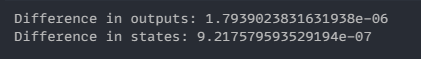
\includegraphics[width=0.4\textwidth]{output2.png}
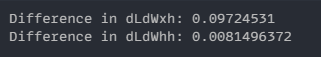
\includegraphics[width=0.4\textwidth]{output1.png}


\section{\normalfont{Becoming Shakespeare (10 pts)}}

For this problem, you will compare a few sequence predictors on Shakespeare's collected works, available from Project Gutenberg. The code to download and preprocess the data is provided in \texttt{ShakespearePrediction.ipynb}. Your task is to implement the following networks (use of \texttt{torch.nn} is highly encouraged):
\begin{enumerate}
    \item A single layer RNN \\
    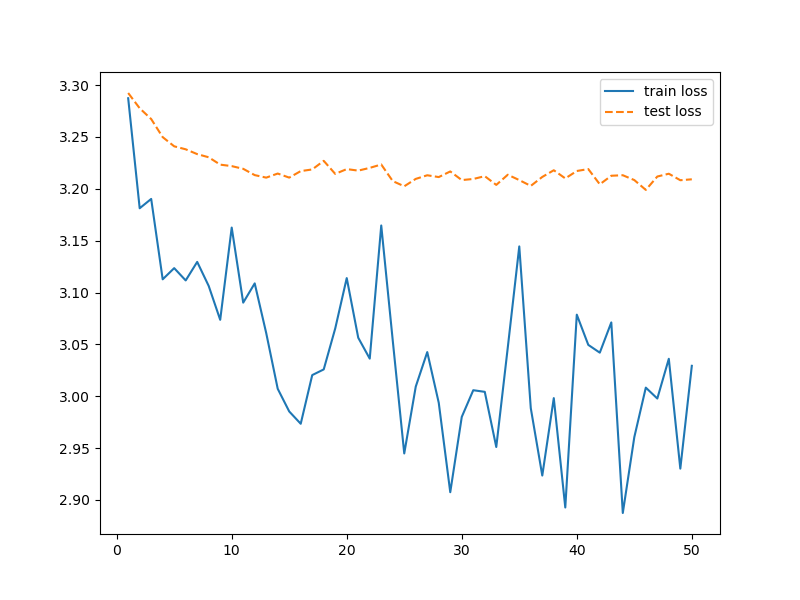
\includegraphics[width=0.4\textwidth]{RNN.png}
    \item A single layer LSTM \\
    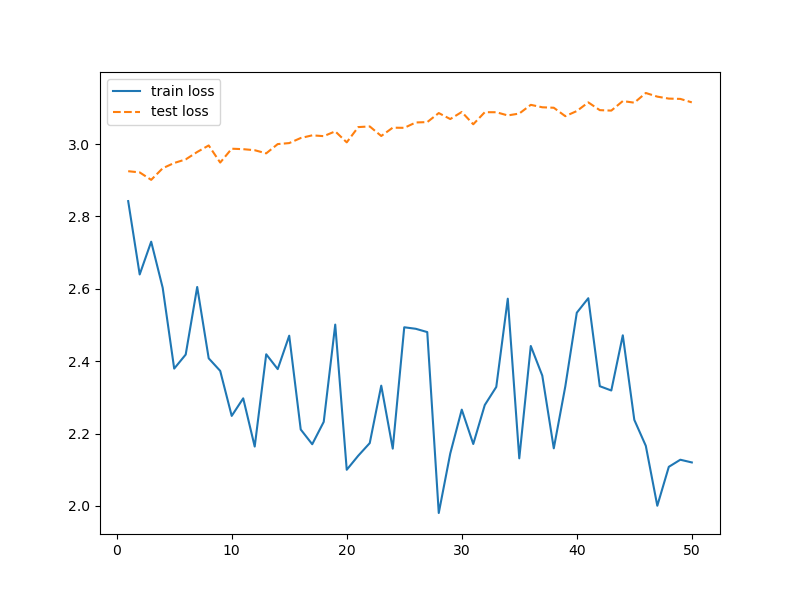
\includegraphics[width=0.4\textwidth]{LTSM.png}
    \item A single layer GRU \\
    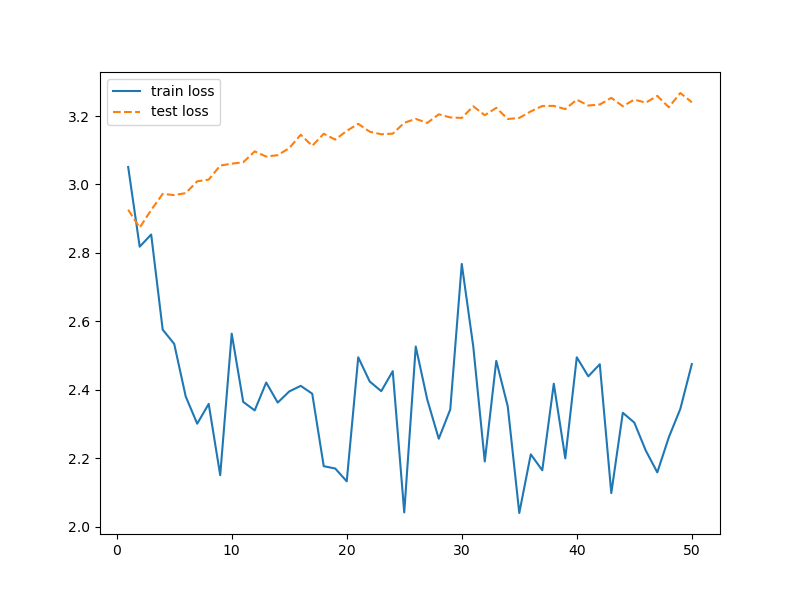
\includegraphics[width=0.4\textwidth]{GRU.png}
    \item One of the above with multiple layers. \\
    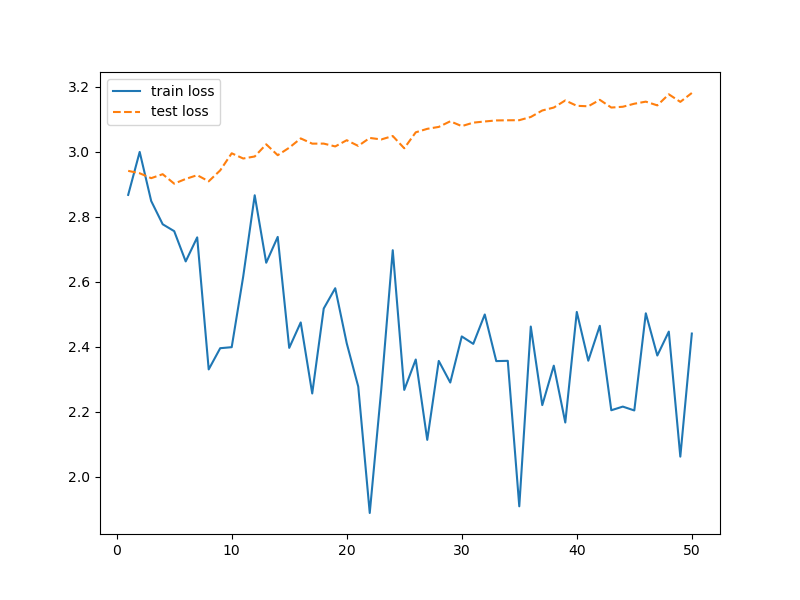
\includegraphics[width=0.4\textwidth]{Multilayer.png}
\end{enumerate}
Turn in the following:
\begin{enumerate}[(a)]
    \item A description of your learning rate, batch size, and any other information needed to replicate your results. \\
    \textbf{Answer:}\\
    Learning rate: 0.01\\
    Batch size: 64\\
    Hidden Size: 64 \\
    Input Length: 5\\
    Output Size: 27\\
    \emph{Note:}Dropout was used, but had little to no effect, so it is not necessary to replicate the results.


    \item Plots showing the training and validation loss versus epoch for each model.
    \textbf{Answer:}\\
    Plots displayed above.
    \item A table comparing the prediction error and perplexity for each of the four models.
    \textbf{Answer:}\\
    \begin{tabular}{|c|c|c|}
        \hline
        Model & Prediction Accuracy & Perplexity \\
        \hline
        RNN & 29.2\% & 19.24 \\
        \hline
        LSTM & 33.2\% & 17.59 \\
        \hline
        GRU & 28.6 & 21.66 \\
        \hline
        Multilayer & 33.1 & 17.22 \\
        \hline
    \end{tabular}

    \item A description of which part of this problem was most challenging for you.
    \textbf{Answer:}\\
    Creating the models was fairly easy. The most difficult part was finding optimal sequence output and input lengths, as well as keeping the model from overfitting. It is fairly obvious from my model graphs that I was unable to remove the overfitting in my graphs, however given more time and perhaps a rework of the model, I believe I could have found a better architecture.
\end{enumerate}

\section{\normalfont{Course Evaluation (3 pts + 50 Lipor pts)}}

You should have received one or more messages requesting that you complete a course evaluation. Please complete this evaluation, and type ``I have completed the course evaluation'' once you've done so. \textbf{Note:} To maintain anonymity, I will not review which students answer affirmatively to this question. \\

I have completed the course evaluation

\section{\normalfont{MP3 Topic (0 pts)}}

As stated in class, the provided problem for MP3 will involve predicting physiological parameters of interest from ultrasound images of eyes. However, since this project does not involve prediction on sequetial data, I am giving you the option to choose a problem of your own to solve for MP3. If you wish to select your own project, it need not be one focused on sequential data, but it must be a problem you have not previously solved. Turn in a description of the problem you wish to solve
or a sentence stating that you'll work on the provided problem for MP3. \\

I will work on the provided problem.

\end{document}